\section{Methodology}
Our methodology is summarized in the workflow illustrated in \textit{Figure~\ref{fig:methods-overview}}.

\begin{figure}[h!]
    \centering
    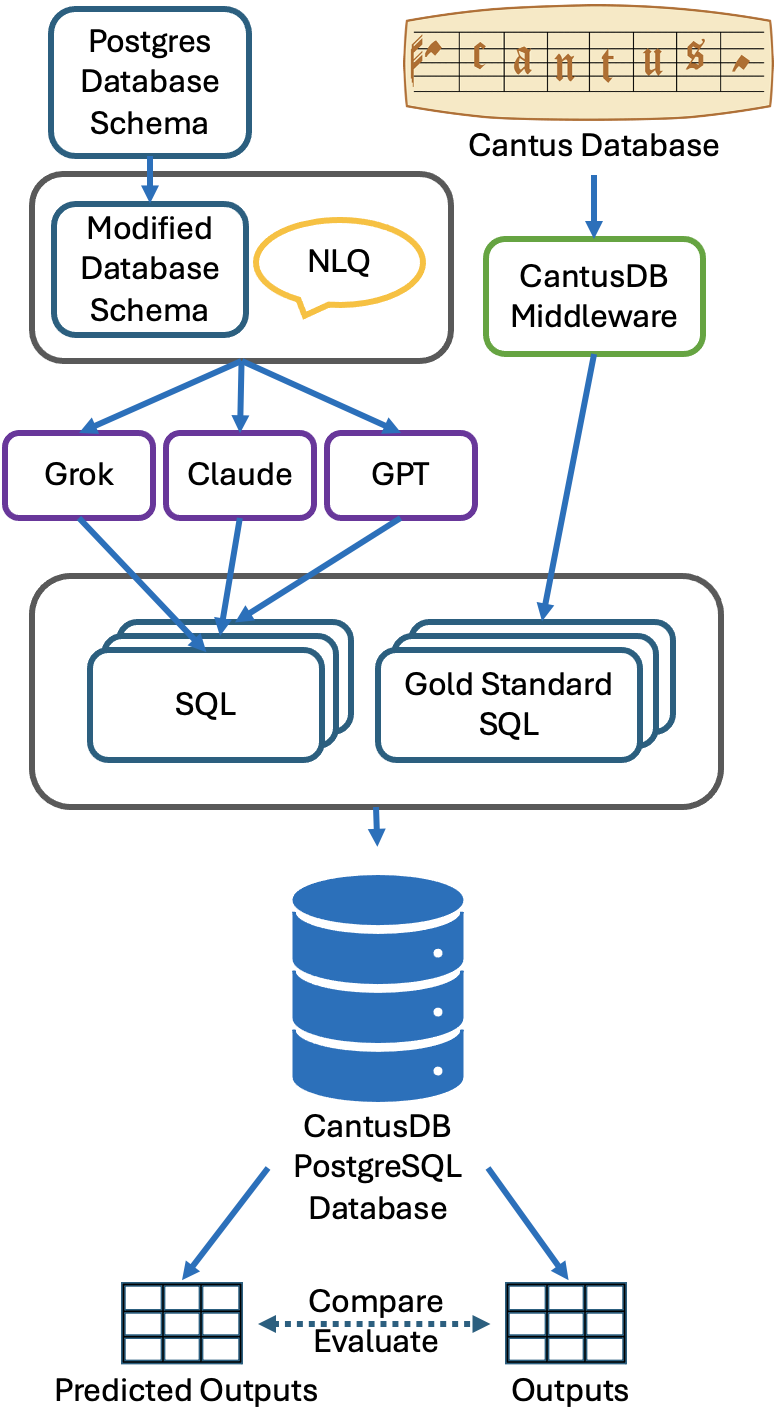
\includegraphics[width=0.35\textwidth]{Figures/methods-workflow.png} % Adjust width as needed
    \caption{Overview of the methodology: Ground truth SQL queries from Cantus Database and natural language queries with a database schema are used to prompt LLMs. The generated SQL queries are executed on the PostgreSQL Cantus Database, and the resulting object IDs are compared and evaluated.}
    \label{fig:methods-overview} % Label for referencing the figure
\end{figure}

\subsection{Overview}
Ground truth data is collected from Cantus Database using a locally deployed version of the website\footnote{Setup instructions are available at \url{https://github.com/DDMAL/CantusDB/wiki}.}. To capture SQL queries made on the database, a custom middleware is integrated into the codebase\footnote{Middleware setup instructions are detailed in the project’s README.md file.}. Additionally, a PostgreSQL database dump is used to extract the database schema. To fit within the context token limits of modern LLMs, the schema is reduced in size and complexity. The details of the reduction process are provided in Section \ref{sec:prompt_engineering}.

Ground truth and predicted data are stored in JSON files, organized by LLM (GPT, Claude, Grok) and object type (\textit{Chants}, \textit{Feasts}, and \textit{Sources}). Each entry includes the gold SQL query, output path, and natural language input. LLMs are prompted with the database schema and queries to generate SQL, which is executed in a PostgreSQL Docker container to produce CSV outputs. Paths to these outputs are recorded alongside the ground truth.

\subsection{Dataset}
The dataset consists of 45 ground truth samples, with 15 samples for each object type (\textit{Chants}, \textit{Feasts}, and \textit{Sources}). Each of the three LLMs generates predictions for 15 natural language input samples per object type, producing a total of 45 predicted SQL queries and corresponding outputs per schema. For both schema variations (with and without options) and all three object types, this totals 135 predicted outputs per schema and 270 combined. This structured approach enables a thorough evaluation of the LLMs' performance across different schema complexities and object types.

\subsection{Prompting Large Language Models}
To generate SQL queries using the LLMs, we create prompts that integrate the modified database schema with natural language inputs. To clearly differentiate values and attributes from regular text, we enclose values in single quotes and capitalize attribute names. An example of such a prompt is:
\begin{quote}
\textit{``Given this database schema, generate a SQL query that shows me all the Sources in the `CANTUS Database' Segment as a Complete Source, from the Country `Germany' and Provenance `Aachen', sorted by institution siglum and source shelfmark. Format your response without any formatting or newlines.''}
\end{quote}

Once the natural language inputs and schemas are finalized, they are provided as prompts to the GPT, Claude, and Grok models. Each LLM generates an SQL query in response to the given prompts. These queries are executed on the PostgreSQL database on CantusDB, producing outputs that include lists of IDs corresponding to the search results for \textit{Chants}, \textit{Sources}, or \textit{Feasts}—objects aligned with the search pages on Cantus Database website. The generated outputs are compared to the ground truth results, i.e., the SQL query outputs obtained directly from the PostgreSQL database. The evaluation methodology, detailed in Section \ref{sec:evaluation_metrics}, combines various techniques to assess the accuracy and usability of the SQL queries generated by the LLMs within the context of Cantus Database.

\subsection{Prompt Engineering}
\label{sec:prompt_engineering}
The LLMs are provided with a modified database schema and a natural language input as context. The schema is generated by systematically processing the PostgreSQL database dump through the following steps:

\begin{enumerate}
    \item Extract the database schema using PostgreSQL's schema-only dump feature.
    \item Filter out only the table creation statements from the schema dump.
    \item Include essential constraints, such as primary keys, foreign keys, and references.
    \item Simplify the schema by removing non-essential modifiers, such as deferrable constraints.
    \item Clean up leading whitespace and other formatting inconsistencies.
    \item Integrate the fixed values into the database schema to produce the extended version.
\end{enumerate}

In the sixth step, we introduce an extended version (with options) of the database schema that includes fixed values relevant for filtering data on Cantus Database website but absent in the raw schema. This extended schema aims to evaluate whether adding such contextual details improves the performance of SQL queries generated by the LLMs. The fixed values are outlined below.
\begin{itemize}
    \item External identifiers for standard metadata repositories: RISM Online, VIAF, Wikidata, GND, Biblioth\`{e}que Nationale de France, Library of Congress, and DIAMM.
    \item Source completeness statuses: Full Source, Fragment, Reconstruction, and Fragmented.
    \item Temporale and Sanctorale prefixes used for Feast filtering.
    \item Proofreading status: Any, Yes, or No.
\end{itemize}

\subsection{Evaluation Metrics}
\label{sec:evaluation_metrics}
Five quantitative evaluation metrics were used to gauge the performance of the different LLMs. The first verified if the SQL queries generated by the LLMs returned the correct elements, ignoring the order. The second metric was the ordered metric, which made sure the items were in the correct order. This was done since Cantus Database search requires the user to specify an order of the items, and this order was reflected in the natural language query. These two metrics were treated as raw counts, so a value of 32 means that 32 out of the 45 queries were correct. Since there are 45 queries in total, both metrics are out of 45.

Precision, recall, and F1 were used to assess the performance. Precision measures how many items the LLM generates are correct, reflecting how well the model avoids generating irrelevant items. Whereas recall evaluates how many correct items from the gold standard were generated by the model, indicating its ability to capture all relevant results. To balance precision and recall, the F1 score was also calculated. The F1 score is the harmonic mean of precision and recall, providing a single metric for correctness and completeness. This is particularly relevant to Cantus Database users, as maximizing precision ensures all results are accurate with no false positives, while high recall guarantees that no relevant items are omitted from the search. The final metric used is the average across the 45 queries.
